\documentclass[parskip=full,11pt,twoside]{scrartcl}
\usepackage[utf8]{inputenc}

\title{Simulator für wiederholte Spiele}
\author{Sebastian Feurer, Peter Koepernik, Luc Mercatoris,\\Christian Schorr, Pierre Toussing}

% section numbers in margins:
\renewcommand\sectionlinesformat[4]{\makebox[0pt][r]{#3}#4}

% header & footer
\usepackage{scrlayer-scrpage}
\lofoot{\today}
\refoot{\today}
\pagestyle{scrheadings}

\usepackage[sfdefault,light]{roboto}
\usepackage[T1]{fontenc}
\usepackage[german]{babel}
\usepackage[yyyymmdd]{datetime} % must be after babel
\renewcommand{\dateseparator}{-} % ISO8601 date format
\usepackage{hyperref}
\usepackage{amsmath} % for $\text{}$
\usepackage[nameinlink]{cleveref}
\crefname{figure}{Abb}{Abb}
\usepackage[section]{placeins}
\usepackage{xcolor}
\usepackage{graphicx}
\hypersetup{
	pdftitle={Pflichtenheft},
	bookmarks=true,
}
\usepackage{csquotes}

\newcommand\urlpart[2]{$\underbrace{\text{\texttt{#1}}}_{\text{#2}}$}

\usepackage{pflichtenheft}

\def\adapt{Adaptionsschritt}
\def\adapts{Adaptionsschritte}

\begin{document}
\maketitle

\section{Einleitung}

Ziel dieses Projekts ist die Entwicklung einer Simulationsumgebung für wiederholte Spiele. Sie ist aus der Forschung motiviert und für den Einsatz in der Forschung ausgelegt. Die Simulationsumgebung wird verwendet, um das Entstehen von Gleichgewichtszuständen bei wiederholten Spielen mehrerer Agenten zu untersuchen. 

Es folgt eine Erläuterung des dem Simulator zugrundeliegenden Ablaufs. Dazu sei auch auf %\cref{} verwiesen.

Eine Simulation besteht aus mehreren Wiederholungen. Eine Wiederholung beginnt mit der Initialisierung der Agenten mit Strategien, Kapital und Gruppenzugehörigkeit. Anzahl der Agenten, Zuweisungsverfahren von Anfangsstrategien und Anfangskapital sowie Gruppeneinteilung werden vom Nutzer spezifiziert. Insbesondere legt der Nutzer die Menge aller möglichen Strategien fest. Danach folgen wiederholt \adapts, bis sich ein Gleichgewicht eingestellt hat oder eine konfigurierbare Höchstzahl an \adapts n erreicht ist. Ein \adapt\ besteht aus einer festen Zahl an Runden. In jeder Runde werden zunächst gemäß eines konfigurierbaren Algorithmus' Paare aus Agenten gebildet. Diese spielen dann gemäß ihrer aktuellen Strategie das dieser Simulation zugrundeliegende Stufenspiel. Nach Ablauf der Runden wird der Erfolg jedes Agenten in den zurückliegenden Runden quantifiziert und daraus eine Rangliste aller Agenten erstellt. Die Agenten passen nun ihre Strategien gemäß eines vom Nutzer spezifizierbaren Adaptionsmechanismus an. Ziel ist dabei nicht die Maximierung des Absolutkapitals, sondern eine möglichst hohe Position auf der Rangliste.

Nachdem alle Wiederholungen abgeschlossen sind, erfolgt die Ausgabe der Ergebnisse der einzelnen Wiederholungen. Wenn sich ein Gleichgewicht eingestellt hat, werden die Zahl der durchgeführten \adapts, die endgültigen Strategien und die endgültige Rangliste ausgegeben.

\pagebreak
\section{Kriterien}
% Diese Section sollte kurz und knapp "für Manager" sein
% und auf eine Seite passen.

\subsection{Muss}

\criterium{Starten einer Simulation}{crt:startsim}	

Der Nutzer kann eine Simulation starten, welche dann mit den aktuell festgelegten Parametern durchgeführt wird.

\criterium{Ausgabe der Simulationsergebnisse}{crt:simresults_std}

Nach Durchführung einer Simulation wird für jede der Wiederholungen ausgegeben, ob sich ein Gleichgewicht eingestellt hat. Falls ja, werden die Zahl der durchgeführten \adapts, die endgültigen Strategien und die endgültige Rangliste ausgegeben.

\criterium{Abbrechen einer Simulation}{crt:interruptsim}

Der Nutzer kann eine laufende Simulation abbrechen.

\criterium{Anpassen von Simulationsparametern}{crt:simparam_std}

Der Nutzer hat die Möglichkeit, die folgenden Simulationsparameter festzulegen:
\begin{itemize} \itemsep -10pt
\item Anzahl der Agenten
\item zugrundeliegendes Stufenspiel
\item Anzahl verschiedener Gruppen und jeweils Anzahl zugehöriger Agenten
\item Zuweisungsverfahren für initiale Strategien
\item Menge aller möglichen Strategien
\item Zuweisungsverfahren für initiales Kapital
\item Algorithmus zur Bildung von Paaren beim Beginn einer Runde
\item Erfolgsquantifizierung zur Erstellung der Rangliste am Ende eines \adapt s
\item Adaptionsmechanismus, nach dem Agenten am Ende eines \adapt s ihre Strategien anpassen
\end{itemize}

\subsection{Kann}

\criteriumOptional{Detailliertere Ausgabe}{crt:simresults_add}
Nach Ablauf einer Simulation können für jede Wiederholung Rangliste und Strategien am Ende aller Adaptionsschritte eingesehen werden.

\criteriumOptional{Anpassen der Abbruchbedingungen}{crt:exitcondition}
Es können mehrere Kriterien für den Abbruch einer Wiederholung verwendet werden.

\criteriumOptional{Erweiterte Gruppenfunktionalität}{crt:groupfunc}
Zuweisungsverfahren für initiales Kapital und initiale Strategien können für jede Gruppe separat festgelegt werden.

\criteriumOptional{Erstellen eigener Strategien}{crt:createstrat}
Es können eigene Strategien erstellt werden.

\criteriumOptional{Erstellen eigener Stufenspiele}{crt:creategame}
Es können eigene Stufenspiele erstellt werden.

\subsection{Abgrenzung}

\criteriumNot{Kein alternativer Simulationsablauf}{crt:not_altsim}
Der zugrundeliegende Ablauf der Simulation, wie in der Einleitung erklärt, kann nicht verändert werden.

\criteriumNot{Keine komplexen Stufenspiele}{crt:not_complexgames}
Als Stufenspiele sind nur solche zugelassen, die sich als \(2 \times 2\) - Bimatrix mit konstanten Auszahlungen darstellen lassen.

\pagebreak
%%%%%%%%%%%%%%
\section{Produkteinsatz}

\section{Produktumgebung}

%%%%%%%%%%%
\section{Funktionale Anforderungen}

\functionality{Schnelle Weiterleitung}{fnc:o1}
\fulfills{crt:fast}

Um zu einer Kurz- die Lang-URLs zu finden,
benutzt der Dienst einen $O(1)$ Mechanismus.
Es wird sichergestellt,
dass mit einer zunehmenden Anzahl von Kurz-URLs im System
das Finden nicht länger dauert.

\functionality{Login-Möglichkeit auf Homepage}{fnc:login}
\fulfills{crt:login}
\fulfills{crt:github}

Auf der Homepage \texttt{http://atu.rl/} sieht ein Besucher
einen \enquote{Login via Facebook} Knopf.
Weitere Knöpfe wie \enquote{Login via Github} sind möglich.
Siehe \cref{fig:homepage}.

\functionality{Auf jeder Seite ist ein Link \enquote{Impressum}}{fnc:impressum-link}
\fulfills{crt:tmg}

Entsprechend Telemediengesetz (TMG) §1
müssen gewisse Informationen über einen Betreiber jederzeit verfügbar sein.
Die inzwischen etablierte Vorgehensweise ist auf allen~(!) Seiten
einen Link mit dem Text \enquote{Impressum} anzubieten.
Dieser Link für auf eine Seite mit entsprechender Erklärung.

\functionality{Auf jeder Seite ist ein Link \enquote{Datenschutz}}{fnc:datenschutz-link}
\fulfills{crt:tmg}

Entsprechend Telemediengesetz (TMG) §13
muss der Betreiber den Nutzer Speicherung und Verarbeitung seiner personenbezogenen Daten unterrichten.
Die inzwischen etablierte Vorgehensweise ist auf allen (!) Seiten
einen Link mit dem Text \enquote{Datenschutz} anzubieten.
Dieser Link für auf eine Seite mit entsprechender Erklärung.

\functionality{Daten werden persistent gespeichert}{fnc:persistence}

Ein geordneter Neustart des Diensts führt nicht zu Datenverlust.

%%%%%%%%%%%
\section{Nicht-Funktionale Anforderungen}

\nonFunctionality{Modernes Design}{nfc:design}

Das Design soll modern und seriös wirken.

\nonFunctionality{Persistenz}{nfc:persistence}

Sollten in Zukunft Erweiterungen oder Updates notwendig werden,
müssen die Daten (Kurz-URLs, E-Mailaddressen) erhalten bleiben.

\nonFunctionality{Erweiterbarkeit}{nfc:extensibility}

Das Produkt muss dahingehend erweiterbar sein,
das die Liste der E-Mail-URL Abbildung von authentifizierten Nutzern
abgerufen werden kann.
Wie das genau implementiert wird, ist nicht Teil dieses Projekts.

%%%%%%%%%%%
\section{Tests}

\test{Kurz-URL Erstellen}{tst:create}
\tests{fnc:login}

\teststep{Besucher \enquote{Zoe Washburne} hat einen Browser geöffnet.}
{Zoe navigiert auf die Homepage \texttt{http://atu.rl/}.}
{Die Homepage wird angezeigt wie in \cref{fig:homepage}.}

\teststep{Zoe hat einen Facebook-Account.}%
{Zoe drückt den \enquote{Login via Facebook} Knopf.}%
{Zoe wird eingeloggt und auf die Erstellseite wie in \cref{fig:form} weitergeleitet.}

\teststep{}
{Zoe befüllt das Feld \enquote{URL} mit \texttt{sehrlangedomain.com/undganzlangeURL.html} und drückt auf \enquote{Kurz-URL erstellen}.}%
{Ihr wird eine Kurz-URL angezeigt wie z.B.\ \texttt{atu.rl/abc}
 wie in \cref{fig:generated}.
 Statt \enquote{abc}, dürfen beliebige andere Buchstaben und Zahl angezeigt werden, allerdings exakt drei.}

\teststep{}
{Zoe navigiert auf die eben generierte Kurz-URL, z.B.\ \texttt{http://atu.rl/abc}.}
{Sie wird zu \texttt{sehrlangedomain.com/undganzlang  eURL.html} weitergeleitet.}

\test{Betreiberinfos lesen}{tst:tmg}
\tests{fnc:impressum-link}
\tests{fnc:datenschutz-link}

\teststep{Besucher \enquote{Jayne Cobb} ist auf der Homepage}
{Er folgt dem Link mit dem Text \enquote{Datenschutz}}
{Ein Text mit allen Datenschutzinformationen wird ihm angezeigt.}

\teststep{}
{Jayne folgt dem Link mit dem Text \enquote{Impressum}}
{Ein Text mit Informationen des Betreibers wird ihm angezeigt.}

%%%%%%%%%%%%%
\pagebreak
\appendix

\section{Seitenentwürfe}

% made via https://gomockingbird.com/projects/mnf0cwf/4gXVnC

\begin{figure}[hb]
%\fbox{
\includegraphics[width=\textwidth]{image/login.png}}
\caption{\label{fig:homepage}
Homepage mit Login-Funktion
}
\end{figure}

\begin{figure}[hb]
%\fbox{
\includegraphics[width=\textwidth]{image/form.png}}
\caption{\label{fig:form}
Formular zur Generierung einer Kurz-URL.
Getestet beispielsweise in \testlink{tst:create}.
}
\end{figure}

\begin{figure}[hb]
%\fbox{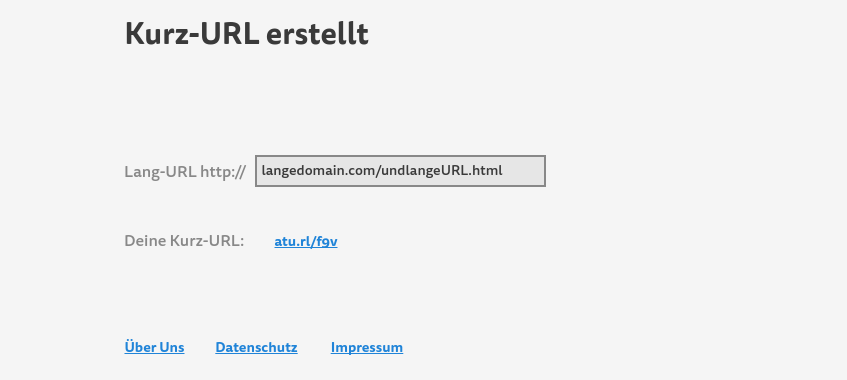
\includegraphics[width=\textwidth]{image/generated.png}}
\caption{\label{fig:generated}
Anzeige der generierten Kurz-URL.
Das Textfeld mit der Lang-URL kann nicht geändert werden.
}
\end{figure}

\section{Glossar}

\textbf{Gleichgewicht}:
Ein Gleichgewicht im Simulationsablauf ist erreicht, wenn keiner der Agenten mehr seine Strategie ändert.

\textbf{Stufenspiel:}
Ein spieltheoretisches Spiel, welches sich als Bimatrix darstellen lässt. (z.B. das Gefangenen-Dilemma)

\textbf{Erfolg:}
Der Erfolg eines Agenten in einer Folge von Runden wird aus dessen Kapitalauszahlungen in diesen Runden berechnet. Er ist Konfigurationsparameter der Simulation. Beispiel ist die Summe aller Auszahlungen.

\textbf{Kapital:}
Jedem Agenten wird im Laufe einer Wiederholung eine Zahl zugeordnet, die sich aus dem Initialisierungswert zu Beginn der Wiederholung und der Summe der Auszahlungen aus den Stufenspielen der bisherigen Runden zusammensetzt.

\textbf{Gruppenzugehörigkeit:}
In einer Simulation sind die Agenten in eine feste, wohldefinierte Anzahl von Gruppen partitioniert. Die Strategien der Agenten können auf die Gruppenzugehörigkeiten anderer Agenten Bezug nehmen.

\textbf{Nutzer}:
Eine Person, welche das Programm nutzt.

\end{document}
